% Copyright 2004 by Till Tantau <tantau@users.sourceforge.net>.
%
% In principle, this file can be redistributed and/or modified under
% the terms of the GNU Public License, version 2.
%
% However, this file is supposed to be a template to be modified
% for your own needs. For this reason, if you use this file as a
% template and not specifically distribute it as part of a another
% package/program, I grant the extra permission to freely copy and
% modify this file as you see fit and even to delete this copyright
% notice. 

\documentclass{beamer}
\mode<presentation> {
    \usepackage[labelformat=empty,
    font=scriptsize,
    skip=0pt,
    justification=centering,
    singlelinecheck=false]{caption}
}
\usepackage[utf8]{inputenc}
\usepackage[backend=biber,style=numeric,sorting=ynt]{biblatex}
\addbibresource{references.bib}

\newcommand\hmmax{0}
\newcommand\bmmax{0}

\renewcommand*{\bibfont}{\tiny}

\graphicspath{{./images/}}

\usepackage{tikz,pgfplots}
\usetikzlibrary{spy}
\pgfplotsset{table/search path={./data}} %checks in data folder
\pgfplotsset{compat=newest}	%mention version to avoid warnings
\pgfplotsset{every axis/.append style={
                    label style={font=\scriptsize},
                    legend style={font=\tiny, draw=none, fill=none},
                    tick label style={font=\small}
                    }}
%To improve the compiling time you can configure the package to export the figures to separate PDF files and then import them into the document
\usepackage{pgfplotstable}
%\usepgfplotslibrary{external}
%\tikzexternalize 
%\usepgfplotslibrary{clickable}
                    
\usepackage[font=scriptsize,labelfont=bf]{caption}
\usepackage[font=scriptsize,labelfont=bf]{subcaption}
\captionsetup[figure]{font=scriptsize,labelfont=scriptsize}
\captionsetup[subfigure]{labelfont=scriptsize,textfont=scriptsize}
\setbeamerfont{itemize/enumerate body}{size=\small}
\usepackage[ngerman,english]{babel}           % switch language

\usepackage{scrtime}                          % gain access to time stamps
%\usepackage{scrpage2}                         % headers and footers
%\usepackage{makeidx}                          % support for makeidx
\usepackage{array}                            % better table support
\newcolumntype{C}[1]{>{\centering\arraybackslash}m{#1}}
\usepackage{multicol}                         % spanning columns
\usepackage{multirow}                         % spanning rows
%\usepackage{amsfonts}
\usepackage{amssymb}
\usepackage{stmaryrd} % for jump in gradient symbol
\usepackage{amsmath, bm, bbm}
\usepackage{mathtools}
\usepackage{relsize}
\usepackage{algorithm}
\usepackage{siunitx}
\usepackage{algpseudocode}
%\usepackage{enumerate}

\usepackage{multimedia}
\usepackage{empheq}
\usepackage[most]{tcolorbox}

\newtcbox{\mymath}[1][]{%
    nobeforeafter, math upper, tcbox raise base,
    enhanced, colframe=blue!30!black,
    colback=blue!30, boxrule=1pt,
    #1}

\setbeamertemplate{bibliography item}{\insertbiblabel}

\setbeamertemplate{itemize item}[ball]
\setbeamertemplate{itemize subitem}[triangle]
\setbeamertemplate{itemize subsubitem}[square]
\setbeamertemplate{enumerate item}[triangle]

\DeclareMathOperator{\erf}{erf}
\DeclarePairedDelimiterX{\norm}[1]{\lVert}{\rVert}{#1}
\newcommand{\seminorm}[1]{\left\lvert #1 \right\rvert}

%\usepackage{hyperref}
%\usepackage{xcolor}


% There are many different themes available for Beamer. A comprehensive
% list with examples is given here:
% http://deic.uab.es/~iblanes/beamer_gallery/index_by_theme.html
% You can uncomment the themes below if you would like to use a different
% one:
%\usetheme{AnnArbor}
%\usetheme{Antibes}
%\usetheme{Bergen}
%\usetheme{Berkeley}
%\usetheme{Berlin}
\usetheme{Boadilla}
%\usetheme{boxes}
%\usetheme{CambridgeUS}
%\usetheme{Copenhagen}
%\usetheme{Darmstadt}
%\usetheme{default}
%\usetheme{Frankfurt}
%\usetheme{Goettingen}
%\usetheme{Hannover}
%\usetheme{Ilmenau}
%\usetheme{JuanLesPins}
%\usetheme{Luebeck}
%\usetheme{Madrid}
%\usetheme{Malmoe}
%\usetheme{Marburg}
%\usetheme{Montpellier}
%\usetheme{PaloAlto}
%\usetheme{Pittsburgh}
%\usetheme{Rochester}
%\usetheme{Singapore}
%\usetheme{Szeged}
%\usetheme{Warsaw}

%\usecolortheme{beaver}

\title[Modelling of Instabilities in MREs]{\small{Master Thesis} \\
\vspace{0.05cm}
\large{Modelling of Instabilities in Magneto-elastic Membranes}}

% A subtitle is optional and this may be deleted
%\subtitle{Master's Project for 10 ECTS}
\vspace{0.25cm}
\author[Vinayak~Gholap]{\footnotesize {Vinayak~Gholap \vspace{0.1cm} \\ supervised by \\Prof.~Dr.-Ing.~habil.~Paul~Steinmann \inst{1}\\Dr.~Jean-Paul~Pelteret \inst{1} \\Dr.~Prashant~Saxena \inst{2}}}
% - Give the names in the same order as the appear in the paper.
% - Use the \inst{?} command only if the authors have different
%   affiliation.

\institute[FAU Erlangen] % (optional, but mostly needed)
{
  \inst{1}
  Chair of Applied Mechanics\\
  Friedrich-Alexander University Erlangen-N\"urnberg, Germany
  \and
  \inst{2}
  University of Glasgow, UK
}
% - Use the \inst command only if there are several affiliations.
% - Keep it simple, no one is interested in your street address.
%\vspace{0.25cm}
\date{\today}
\titlegraphic{
\includegraphics[width=2cm]{ltm.png}\hspace*{4cm}~%
   
\includegraphics[width=3.75cm]{logo_fau.jpg}}
% - Either use conference name or its abbreviation.
% - Not really informative to the audience, more for people (including
%   yourself) who are reading the slides online

\subject{Theoretical Computer Science}
% This is only inserted into the PDF information catalog. Can be left
% out. 

% If you have a file called "university-logo-filename.xxx", where xxx
% is a graphic format that can be processed by latex or pdflatex,
% resp., then you can add a logo as follows:

%\logo{\pgfdeclareimage[width=1cm]{department-logo}{ltm.png}
%\pgfuseimage{department-logo}
%\hspace{\dimexpr\paperwidth-3cm-12pt}
%\pgfdeclareimage[height=1cm]{university-logo}{logo_fau.jpg}
%\pgfuseimage{university-logo}
%}

% Delete this, if you do not want the table of contents to pop up at
% the beginning of each subsection:
\AtBeginSection[]
{
\begin{frame}{Outline}
\tableofcontents[currentsection]
\end{frame}
}
\AtBeginSubsection[]
{
  \begin{frame}<beamer>{Outline}
    \tableofcontents[currentsection,currentsubsection]
  \end{frame}
}

\setbeamercovered{transparent}

% Let's get started
\begin{document}
\tikzstyle{every picture}+=[remember picture]
\addtobeamertemplate{block begin}{\setlength\abovedisplayskip{0pt}}

\begin{frame}
  \titlepage
\end{frame}

\begin{frame}{Outline}
  \tableofcontents
  % You might wish to add the option [pausesections]
\end{frame}

% Section and subsections will appear in the presentation overview
% and table of contents.
\section{Introduction}
\begin{frame}{Introduction}
\begin{itemize}
\item Magneto-active materials: Smart materials of the future!
\item Multi-physics/Coupled problem of magnetic field and non-linear elasticity
\item Non-linear elastic membranes exhibit instabilities under finite loads (elastic limit-point instability)
\end{itemize}

\begin{figure}[h]
\centering 
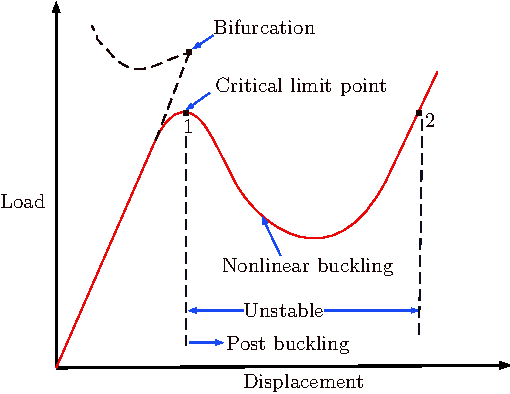
\includegraphics[width=0.5\textwidth]{nonlinear_eq_path.pdf}
\caption{Equilibrium paths for non-linear instability}
\end{figure}
\end{frame}

\begin{frame}{Motivation}
\begin{itemize}
\item Recent research carried in \cite{reddy_toroid,Reddy2018} for magneto-rheological elastomers (MREs) with axisymmetric geometries under inflating pressure loads
\item Occurrence of bulging and wrinkling instabilities in MRE membranes was shown
\item Applied external magnetic load alters the elastic limit point and gives rise to multiple equilibrium states
\item Finite difference method used for the solutions of the resulting coupled ODEs 
\end{itemize}
\begin{columns}
\begin{column}{0.28\textwidth}
\begin{figure}
\centering
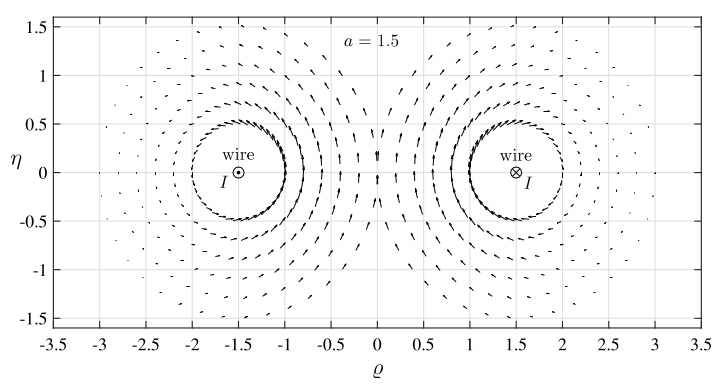
\includegraphics[width=0.98\textwidth]{magnetic_field_saxena.png}
\caption{Experiment set up \cite{reddy_toroid}}
\end{figure}
\end{column}
\begin{column}{0.28\textwidth}
\begin{figure}
\centering
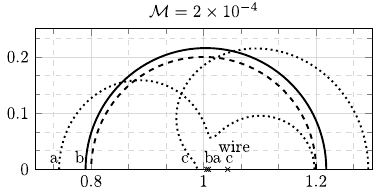
\includegraphics[width=0.98\textwidth]{torus_deformed.png}
\caption{Deformations of torus membrane \cite{reddy_toroid}}
\end{figure}
\end{column}
\begin{column}{0.43\textwidth}
\begin{figure}
\centering
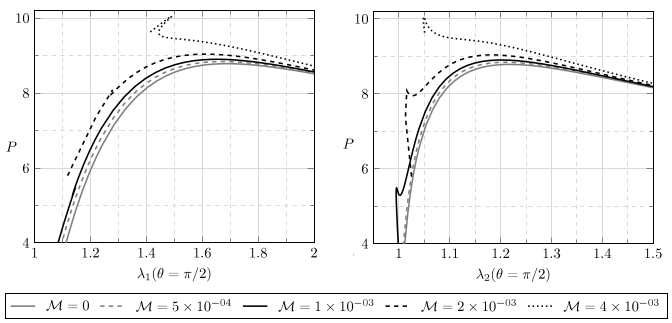
\includegraphics[width=0.98\textwidth]{saxena_load_disp.png}
\caption{Equilibrium paths \cite{reddy_toroid}}
\end{figure}
\end{column}
\end{columns}
\end{frame}

\begin{frame}{Research objectives}
\begin{itemize}
\item Develop a robust multi-physics framework for the magneto-elasticity problems
\item Numerical modelling of thin magneto-elastic membrane near limit points under unstable conditions
\item Model the thin torus shaped membrane along with surrounding free space
\item Axisymmetric formulation to reduce the computational cost
\item Robust scientific implementation using open source C++ FEM library \texttt{deal.II} \cite{dealII90} employing hp-adaptive FEM \& HPC
\end{itemize}
\end{frame}

\section{Implementation details and results}
\subsection{Decoupled problems}
%\subsubsection{Magneto-static problem}

\begin{frame}{Kinematics}
\begin{columns}
\begin{column}{0.4\textwidth}
\begin{itemize}
\item $\mathcal{D}_0 := \mathcal{B}_0 \cup \ \mathcal{S}_0$
\item Gradient w.r.t. $\mathcal{D}_0$: $\nabla_0 \left\lbrace \cdot \right\rbrace$
\item Total Lagrangian formulation employed
\end{itemize}
\end{column}
\begin{column}{0.59\textwidth}
\begin{figure}[h]
\centering
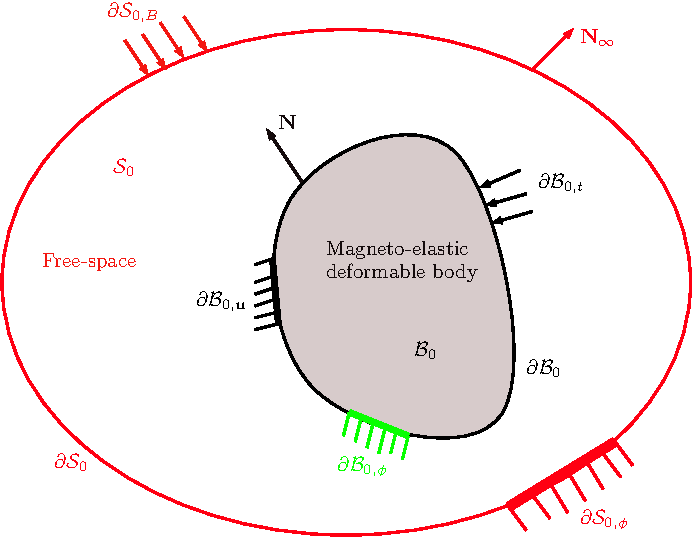
\includegraphics[width=0.9\textwidth]{kinematics_potato_coupled.pdf}
\caption{Domain definition for the deformable magneto-elastic membrane $\mathcal{B}_0$ immersed in an electromagnetically permeable free space $\mathcal{S}_0$.}
\end{figure}
\end{column}
\end{columns}
\end{frame}

\begin{frame}{Magneto-static magnetic scalar potential}
\only<1-3>{
\begin{itemize}
\uncover<1-3>{
\item Magnetic vector fields: $\mathbb{H}, \mathbb{B}, \mathbb{M}$ with $J^{-1} \mathbf{C} \cdot \mathbb{B} = \mu_0 (\mathbb{H} + \mathbb{M})$
\item Modelling with $\mathbb{H}$ as independent field: $\mathbb{B} = \mathbb{B}(\mathbb{H})$
\item Balance law in magneto-statics: $\text{Div}(\mathbb{B}) = 0$ in $\mathcal{D}_0$
}%
\uncover<2-3>{
\item Scalar magnetic potential formulation: $\mathbb{H} := -\nabla \phi$
\item Continuity condition: $\llbracket \phi \rrbracket = 0$
}%
\uncover<3>{
\item Resulting Laplace PDE: $-\mu_0 \mu_r \left(\nabla \cdot \nabla \phi \right) = 0$ in $\mathcal{D}_0$
\item Boundary conditions: $\phi = \overline{\phi}$ on $\partial \mathcal{S}_{0,\phi}$,
$\mathbf{N} \cdot \llbracket \mathbb{B} \rrbracket = \overline{b}$ on $\partial \mathcal{S}_{0,B}$
}%
\end{itemize}
}%
\only<4>{
Axisymmetric problem geometry: Mesh generated using CUBIT \cite{cubit}.
\begin{figure}[h]
\centering
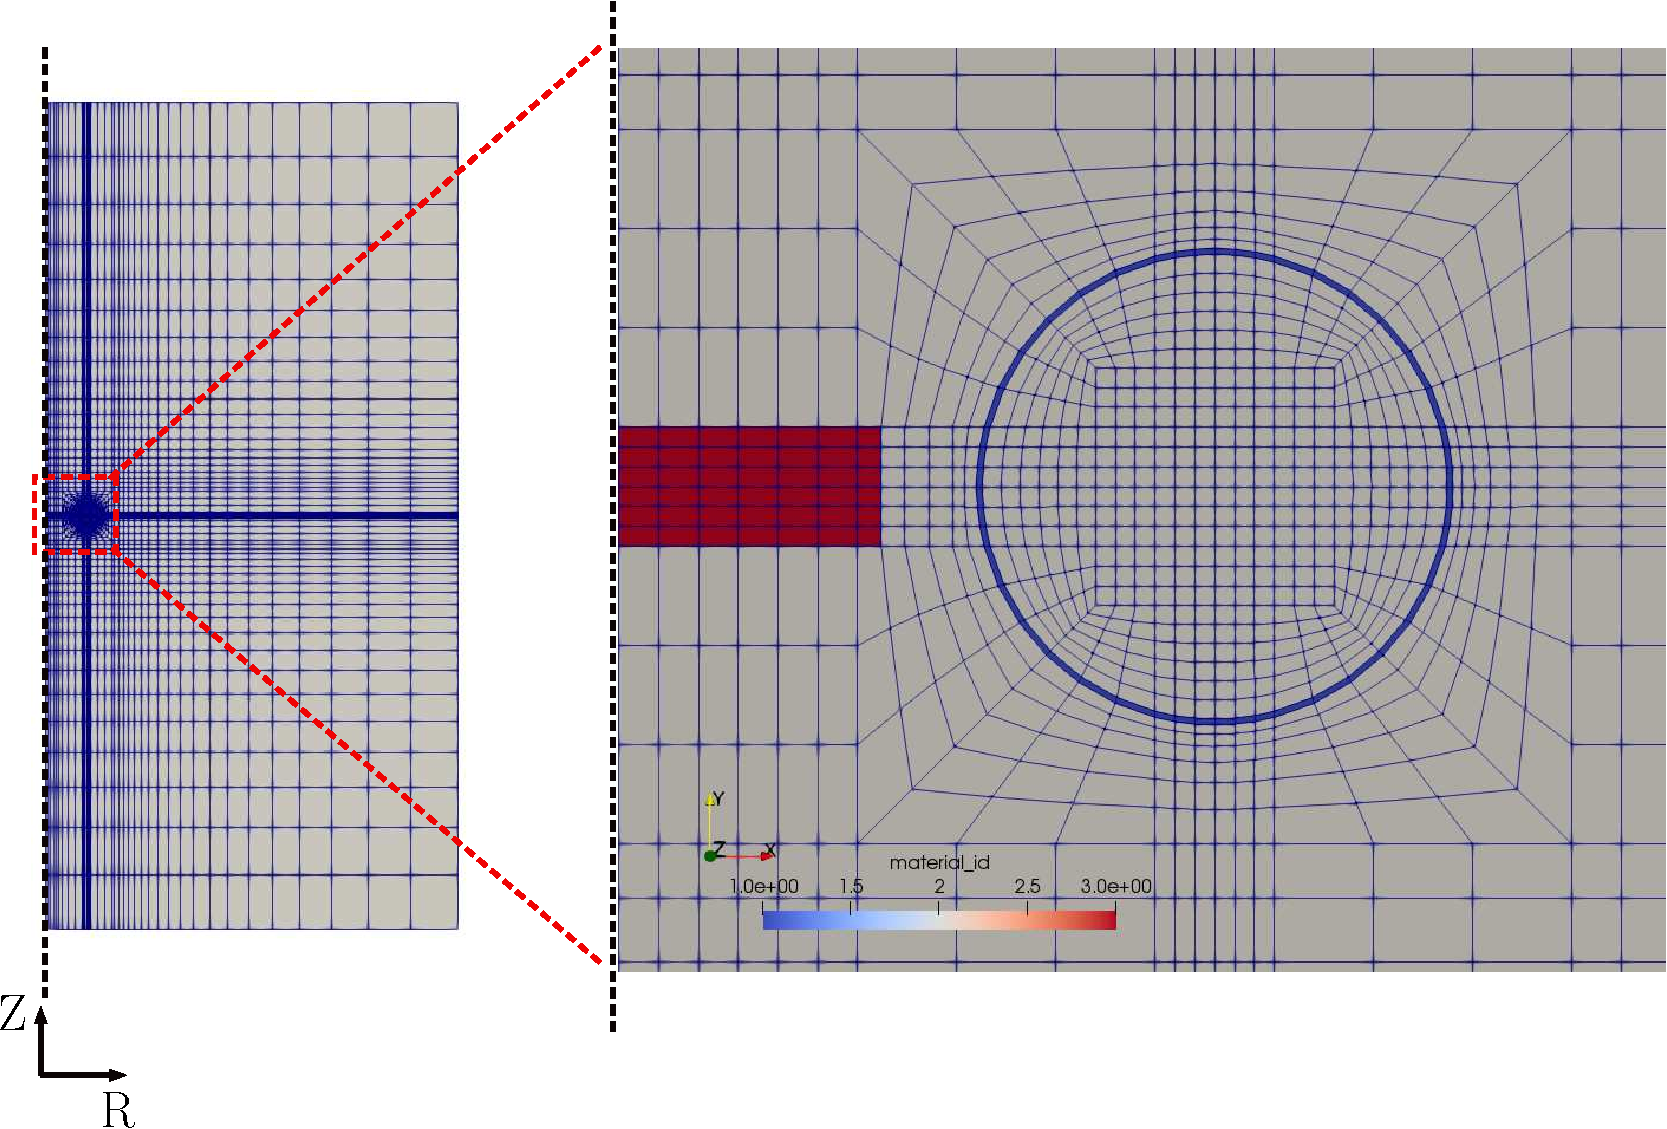
\includegraphics[width=0.8\textwidth]{2d_mesh.pdf}
\caption{Axisymmetric (2.5D) mesh geometry of toroid tube material modelled with surrounding free space (Red region: permanent magnet, blue region: torus magneto-elastic material and remaining region is the free space)}
\end{figure}
}%
\only<5>{
Results:
\begin{columns}
%\onslide<1-3>{
\begin{column}{0.49\textwidth}
\begin{figure}[h]
\centering
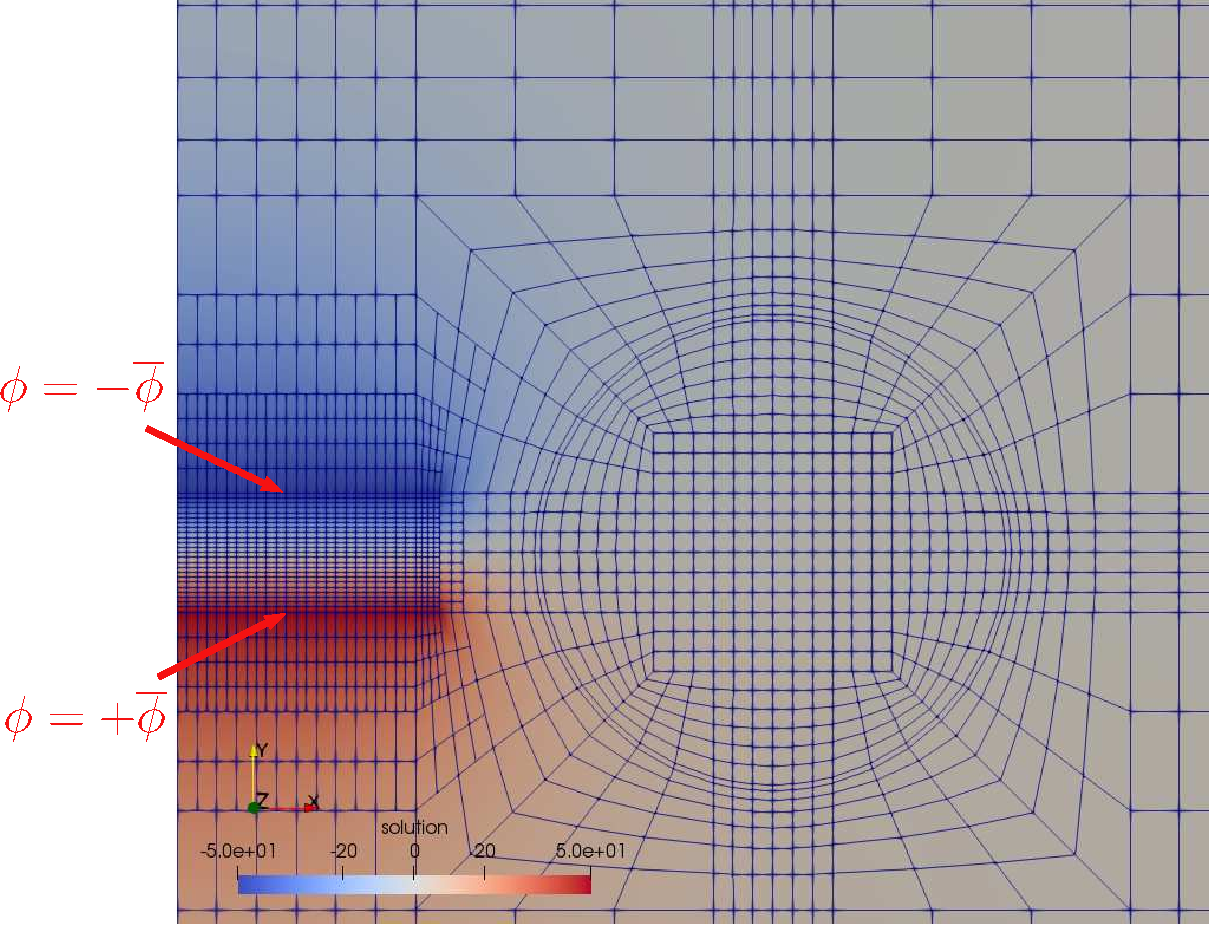
\includegraphics[width=0.6\textwidth]{applied_mag_pot_magnet.pdf}
\caption{Boundary condition for $\phi$}
%}%
\vspace{0.1cm}
%\onslide<3>{
\centering
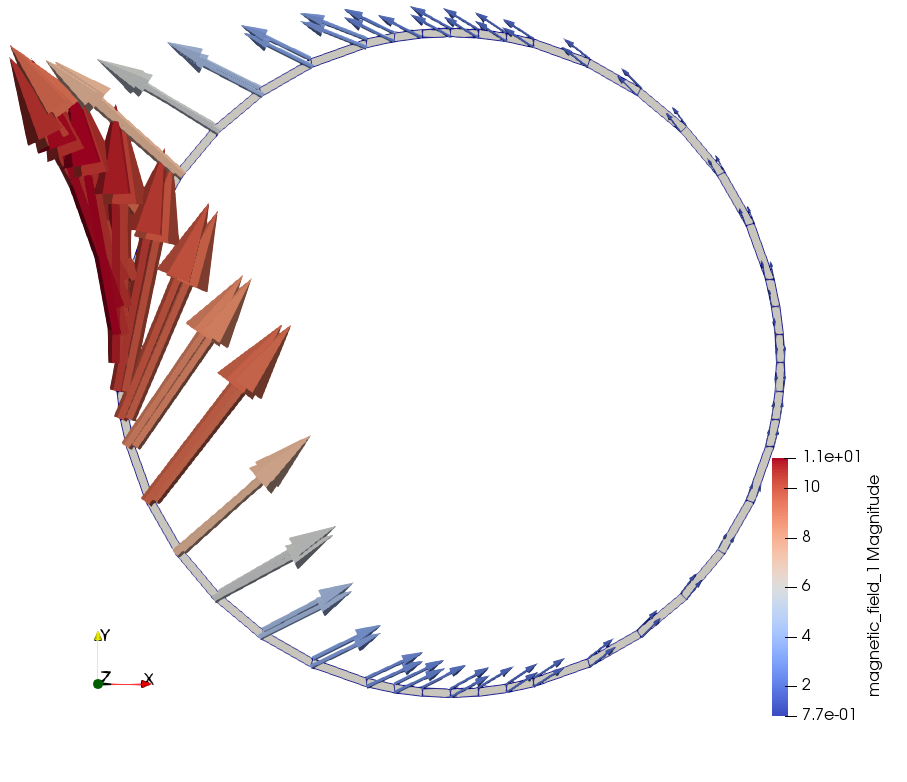
\includegraphics[width=0.6\textwidth]{x_p.png}
\caption{Magnetic field in membrane}
\end{figure}
\end{column}
%}%
%\onslide<2-3>{
\begin{column}{0.49\textwidth}
\begin{figure}[h]
\centering
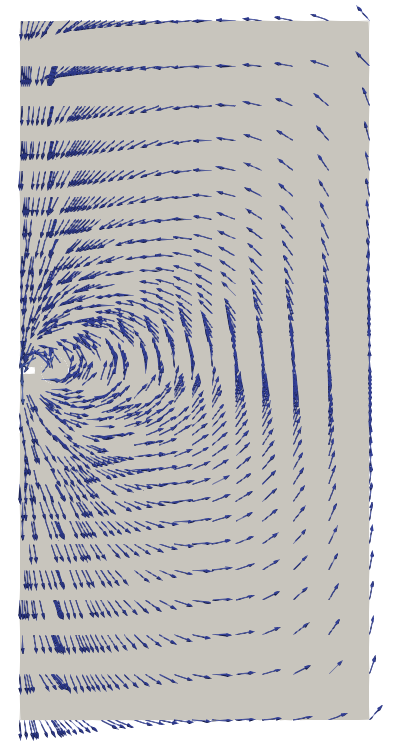
\includegraphics[width=0.6\textwidth]{2d_free_space.png}
\caption{Developed circulating magnetic field (vectors not scaled)}
\end{figure}
\end{column}
%}%
\end{columns}
}%
\only<6>{
3D geometry:
\begin{figure}[h]
\centering
\begin{subfigure}[b]{0.39\textwidth}
\centering
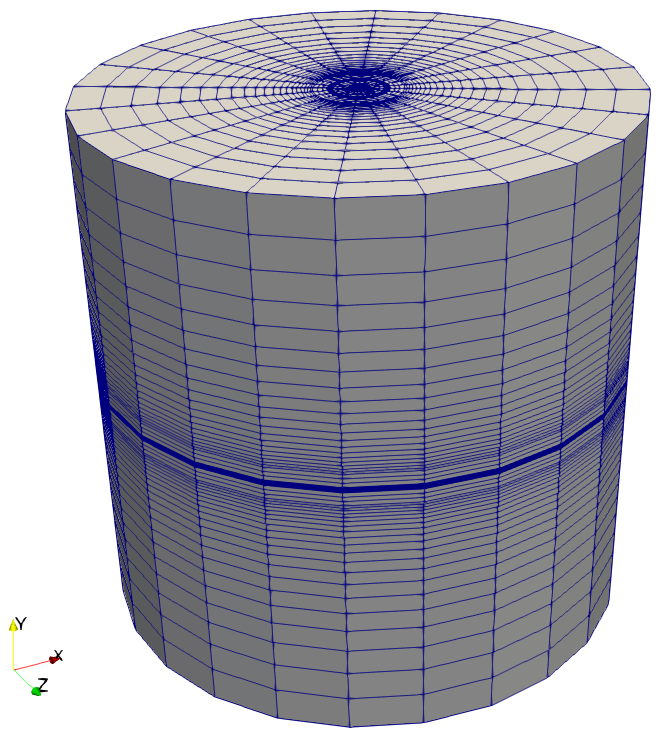
\includegraphics[width=0.9\textwidth]{3d_mesh_1.png}
\caption{3D mesh with free space}
\end{subfigure}
\begin{subfigure}[b]{0.29\textwidth}
\centering
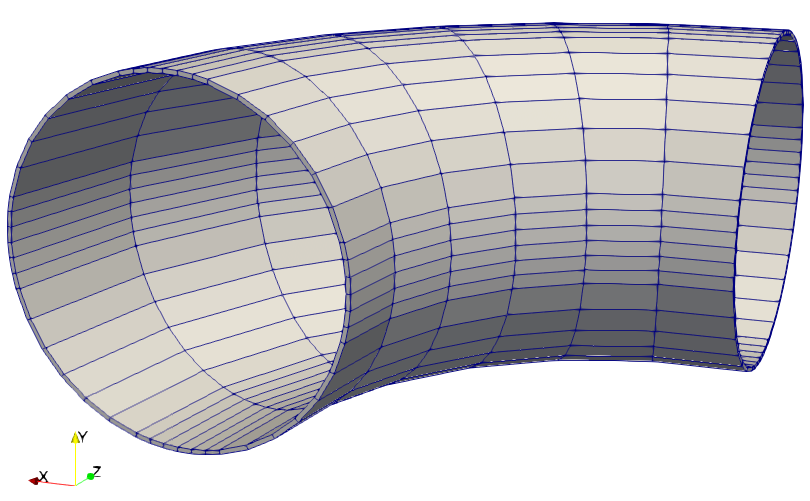
\includegraphics[width=0.85\textwidth]{3d_mesh_3.png}
\caption{Cut section of toroid tube}
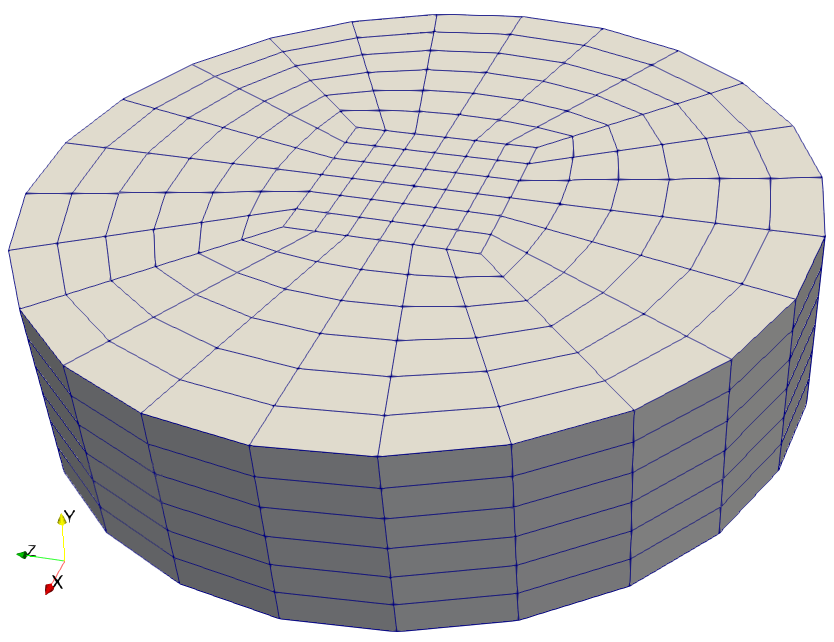
\includegraphics[width=0.85\textwidth]{3d_mesh_5.png}
\caption{Permanent magnet region}
\end{subfigure}
\begin{subfigure}[b]{0.29\textwidth}
\centering
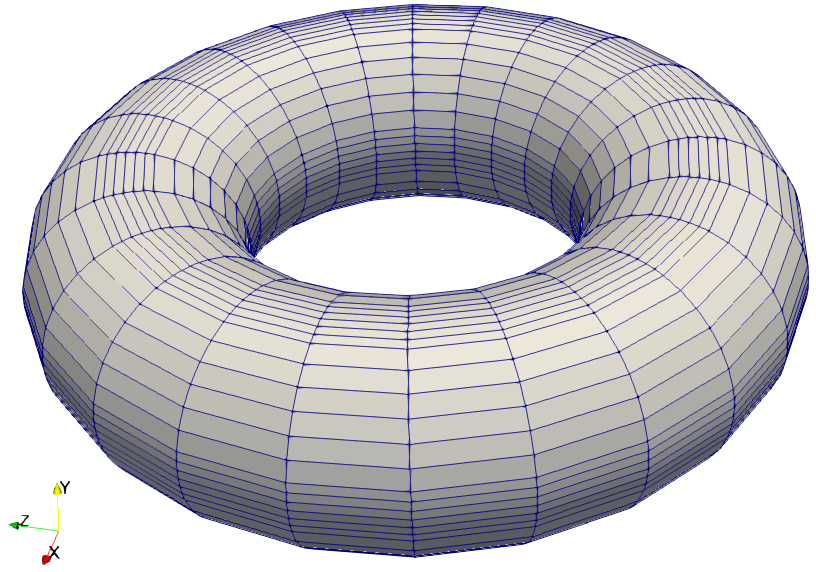
\includegraphics[width=0.75\textwidth]{3d_mesh_4.png}
\caption{Toroid tube}
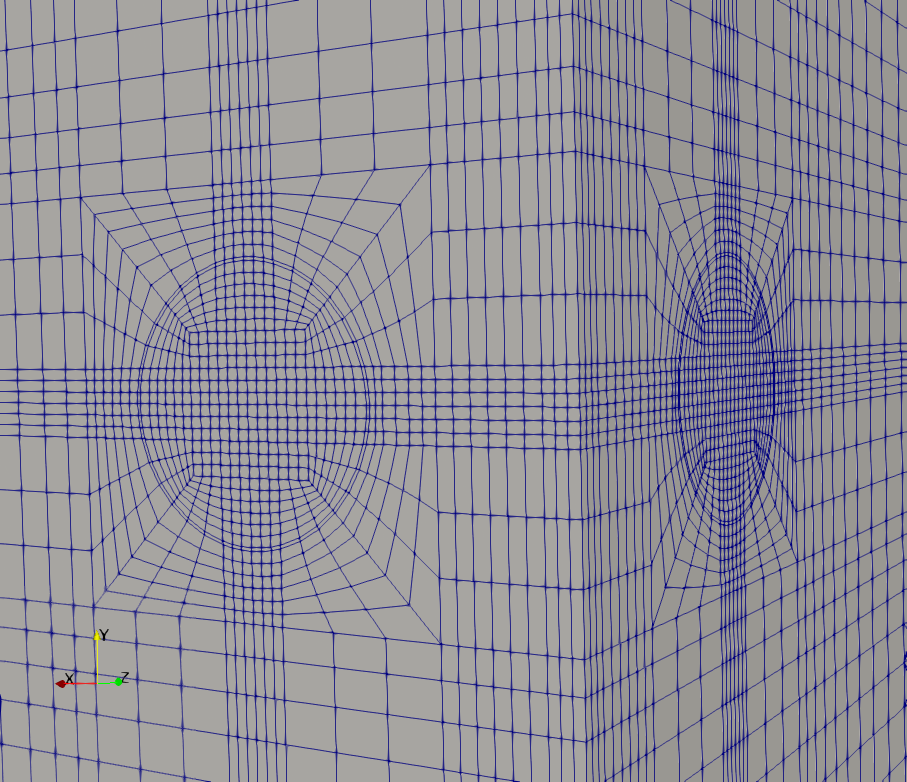
\includegraphics[width=0.75\textwidth]{3d_mesh_6.png}
\caption{Zoomed cross-section}
\end{subfigure}
\caption{3D mesh geometry}
\end{figure}
}%
\only<7>{
\begin{block}{Validation of axisymmetric formulation:}
Energy $E = \sum\limits_{\mathcal{B}_0} \sum\limits_{q} \frac{1}{2} \mu_0 \ \mu_r \ \alpha \ \norm{-\nabla \phi(q)}^2 \ J \ w(q)$, \\
$\alpha = 2 \pi R$ is co-ordinate scaling factor.
\end{block} 
\begin{figure}[t!]
\begin{subfigure}[t]{0.4\linewidth}
\centering
\resizebox{\linewidth}{!}{
\begin{tikzpicture}
\begin{semilogxaxis}[
xlabel = $\text{\small{Number of elements}}$,
ylabel = $\text{\small{Total energy in membrane}}$,
legend pos=north east,
]
\addplot[
color=red,
mark=square,
line width=1pt,
]
table[x=NumberOfCells,y=TotalEnergy]{ref_sol_2d_energy_ncells.dat};
\addlegendentry{\small{Total energy}}
\end{semilogxaxis}
\end{tikzpicture}
}
\caption{Axisymmetric (2.5D)}
\end{subfigure}
\begin{subfigure}[t]{0.37\linewidth}
\centering
\resizebox{\linewidth}{!}{
\begin{tikzpicture} 
\begin{semilogxaxis}[
xlabel = $\text{\small{Number of elements}}$,
legend pos=north east,
]
\addplot[
color=red,
mark=square,
line width=1pt,
]
table[x=NumberOfCells,y=TotalEnergy]{3d_3ref_energy_ncells.dat};
\addlegendentry{\small{Total energy}}
\end{semilogxaxis}
\end{tikzpicture}
}
\caption{3D}
\end{subfigure}
\caption{Comparison of total magnetic energy in the magneto-elastic torus membrane for each h-adaptive refinement cycle \alert{(Relative error $\approx 15\%$)}}
\end{figure}
}%
\end{frame}

%\subsubsection{Compressible finite-strain elasticity problem}
\begin{frame}{Quasi-static non-linear compressible elasticity}
\only<1>{
\begin{itemize}
\item Quantities from non-linear continuum theory: $\mathbf{u},\mathbf{F},\mathbf{C},\mathbf{E}$
\item Balance law: $\text{Div}(\mathbf{F} \cdot \mathbf{S}) + \mathbf{b}^p = \mathbf{0}$ in $\mathcal{D}_0$
\item Constitutive relation: $\mathbf{S} := 2\dfrac{\partial \Psi}{\partial \mathbf{C}}$, \ $\Psi$: Helmholtz free energy density
\item Boundary condition: $\mathbf{u} = \mathbf{0}$ on $\partial \mathcal{S}_{0,\mathbf{u}}$, $ \llbracket \mathbf{F} \cdot \mathbf{S} \rrbracket \cdot \mathbf{N} = \mathbf{t}^p$ on $\partial\mathcal{B}_{0,t}$
\item Vector-valued solution field: $\mathbf{u} = \{ u_r, u_z\}$ in 2.5D problem
\end{itemize}
}%
\only<2>{
\begin{itemize}
\item Transformations needed for axisymmetric formulation:
\begin{align*}
\int\limits_{\mathcal{B}_0} \mathrm{d} V &= \int\limits_{X} \int\limits_{Y} \int\limits_{Z} \mathrm{d} Z \ \mathrm{d} Y \ \mathrm{d} X = \int\limits_{R} \int\limits_{\Theta} \int\limits_{Z} \mathrm{d} Z \ R \mathrm{d} \Theta \ \mathrm{d} R, \nonumber \\
\text{with} \ \int\limits_{\Theta} \mathrm{d} \Theta &= 2 \pi \implies \int\limits_{\mathcal{B}_0} \mathrm{d} V = \int\limits_{R} \int\limits_{Z} 2 \pi \ R \ \mathrm{d} R \ \mathrm{d} Z
\end{align*}
\item For torsionless axisymmetric problem: 
\begin{equation*}
\mathbf{F} = \begin{bmatrix}
r_{, R} & r_{, Z} & 0 \\
z_{, R} & z_{, Z} & 0 \\
0 & 0 & r/R
\end{bmatrix} = \begin{bmatrix}
(1 + u_{r, R}) & u_{r, Z} & 0 \\
u_{z, R} & (1 + u_{z, Z}) & 0 \\
0 & 0 & (1 + u_r / R)
\end{bmatrix}
\end{equation*}
\item Magnetic vector field:
\begin{align*}
\mathbb{H} = \begin{bmatrix}
-\phi_{,R} \\
-\phi_{,Z} \\
0
\end{bmatrix}
\end{align*}
\end{itemize}
}%
\only<3>{
\begin{itemize}
\item Hyperelastic material response characterized by a Helmholtz free energy function $\Psi = \Psi(\mathbf{C})$
\item Neo-Hookean material law used for non-linear rubber-like materials:
\begin{empheq}[box=\tcbhighmath]{align*}
\Psi (\mathbf{C}) \equiv \dfrac{\mu}{2} [\mathbf{C} : \mathbf{I} - \mathbf{I} : \mathbf{I} - 2 \ln J] + \dfrac{\lambda}{2} (\ln J)^2
\end{empheq}
where $\mu$ and $\lambda$ are the Lam\'e parameters
\item Constitutive relation $\mathbf{S} := 2\dfrac{\partial \Psi (\mathbf{C})}{\partial \mathbf{C}}$ \\
\item Referential elastic tangent $\mathfrak{C} := 2 \dfrac{\partial \mathbf{S}(\mathbf{C})}{\partial \mathbf{C}} = 4 \dfrac{\partial^2 \Psi (\mathbf{C})}{\partial \mathbf{C} \otimes \partial \mathbf{C}}$
\end{itemize}
}%
\only<4>{
\begin{columns}
\begin{column}{0.4\textwidth}
\begin{block}{Inflating pressure load:}
$\mathbf{t}^p = \mathbf{P}\mathbf{N} = \left[ p_0 \mathbf{I} \right] \mathbf{N} = p_0 \mathbf{N}$,
\end{block}
$\mathbf{P}$: first Piola-Kirchhoff stress, \\$p_0$: inflating pressure load (scalar), \\$\mathbf{N}$: referential unit normal vector.
\end{column}
\begin{column}{0.59\textwidth}
\begin{figure}[h]
\centering
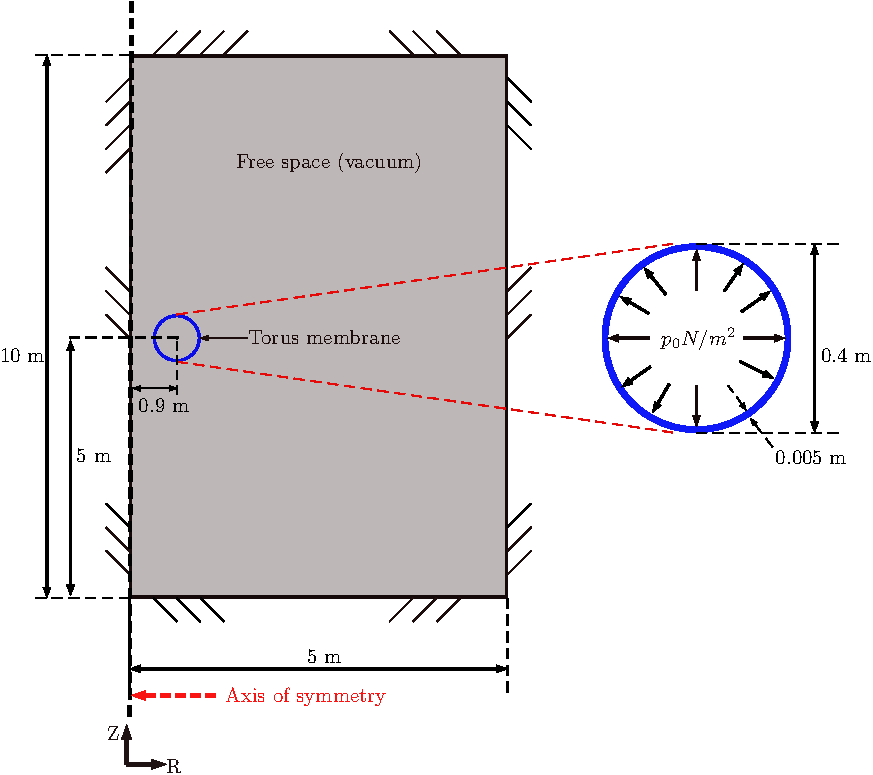
\includegraphics[width=0.85\textwidth]{torus_membrane_grid.pdf}
\caption{Representative geometry}
\end{figure}
\end{column}
\end{columns}
}%
\only<5>{
Resulting deformation for $p_0$ = 1000 Pa.
\begin{figure}[h]
\centering 
\movie[width=8cm,height=7cm,poster,showcontrols]{}{new_finite_deform_torus_elas.avi}
\caption*{Inflating magneto-elastic membrane \alert{(Click image!)}}
\end{figure}
}%
\only<6>{
\alert{Parametric study of free space parameter $\mu$:}
\begin{table}[h]
\centering
\begin{tabular}[c]{|C{3cm}|C{4cm}|C{3cm}|}
\hline
\textbf{Material domain} & \textbf{Shear modulus} $\mu$ (Pa) & \textbf{Poisson ratio} $\nu$ \\
\hline
Membrane & $3e^4$ & 0.4 \\
\hline
Free space & $3e^1 - 3e^{-2}$ & 0.3 \\
\hline 
\end{tabular} 
%\caption{Material parameter values}
\end{table}

\begin{figure}[h]
\centering 
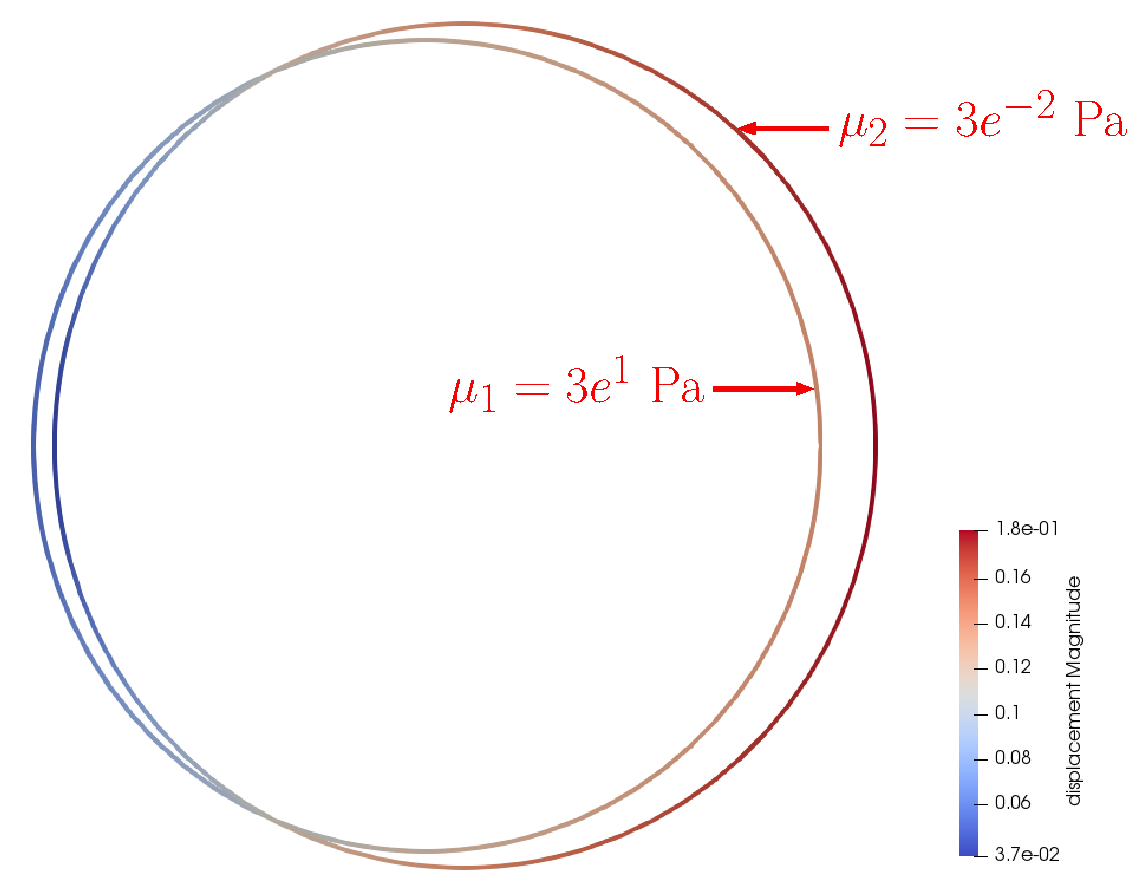
\includegraphics[width=0.5\textwidth]{mue_study_1e3_vs_1e6_full_load.pdf}
\caption{Deformed torus membrane for different free space material parameter $\mu$}
\end{figure}
}%
\end{frame}

%\begin{frame}{Buckling instability in a test problem}
%\only<1>{
%\begin{figure}[h]
%\centering
%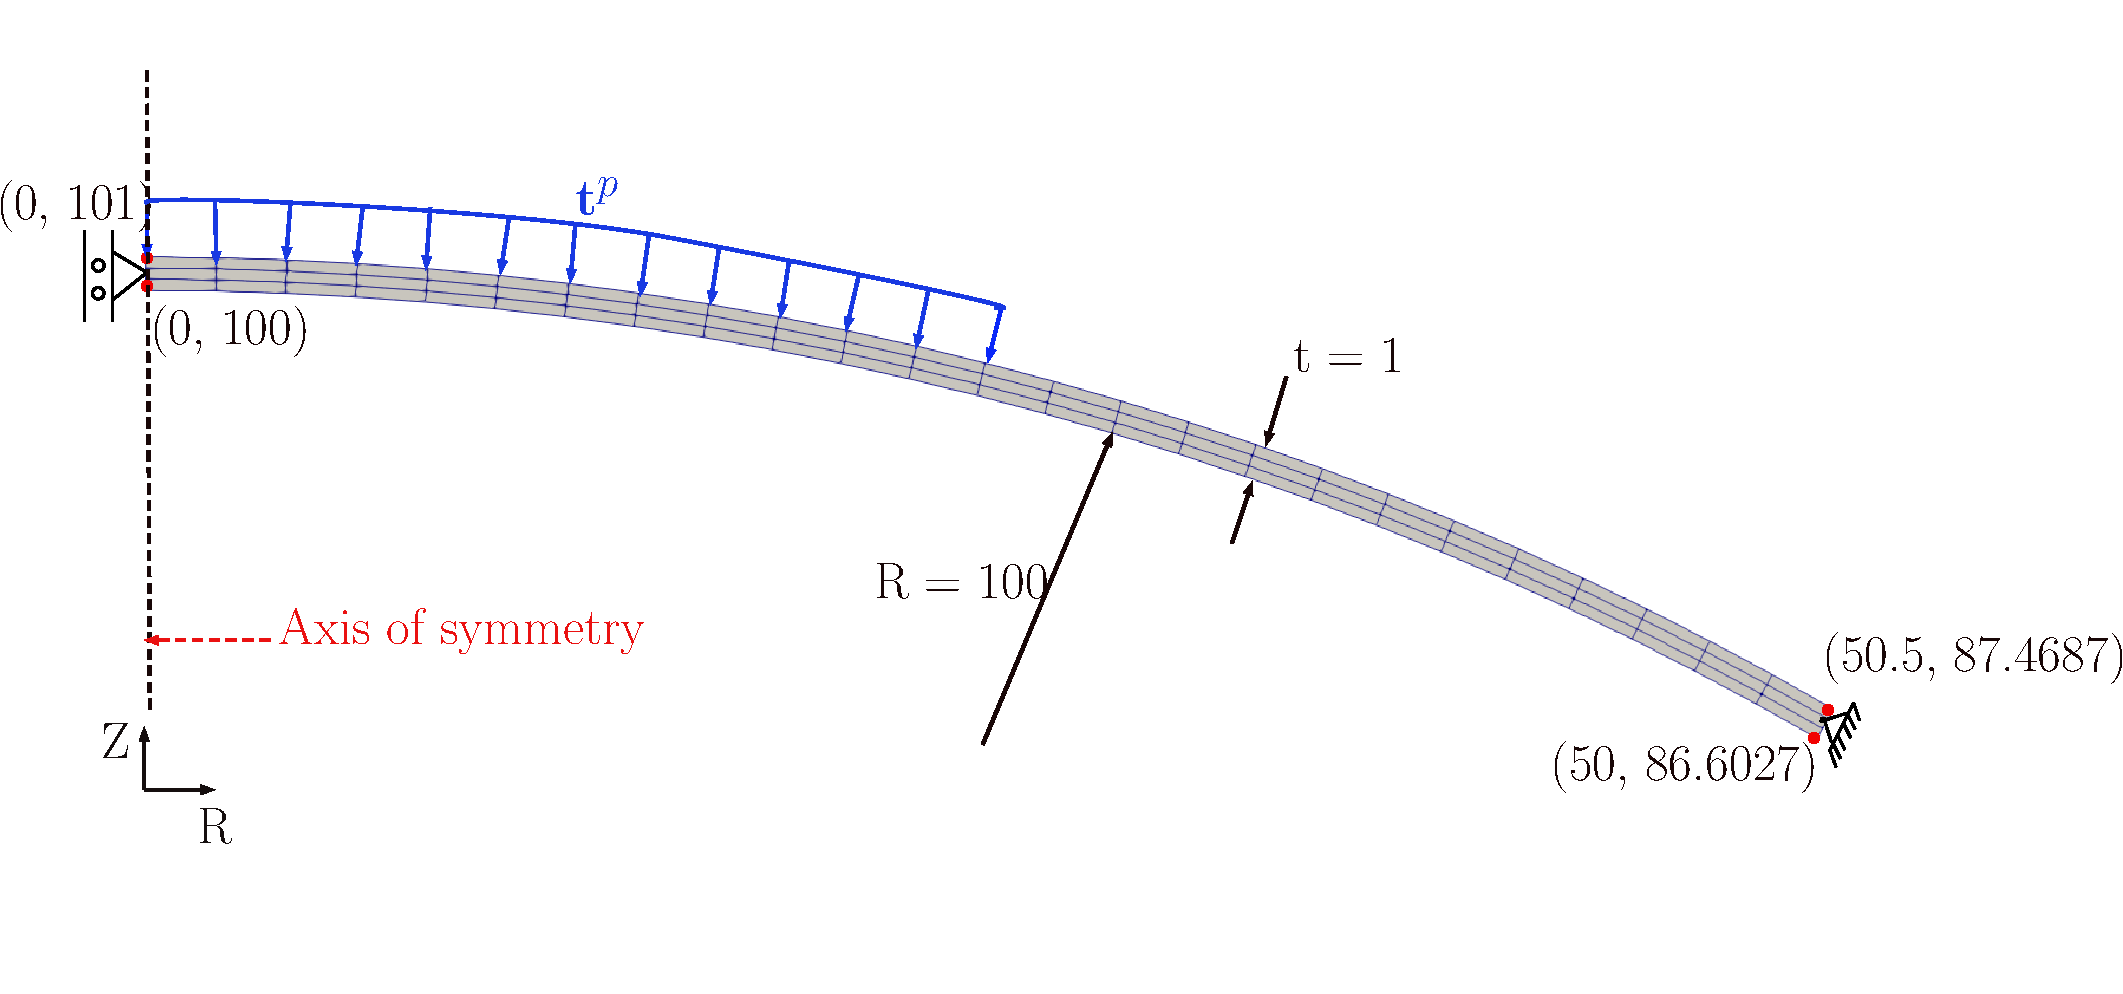
\includegraphics[width=0.7\textwidth]{crisfield_beam.pdf}
%\caption{Crisfield beam test model}
%\end{figure}
%Chosen parameter values for test: $\mathbf{t}^p$ = $2e^{-4} \ \dfrac{\text{N}}{\text{m}}$, $\mu$ = $3e^{-2}$ Pa, $\nu$ = 0.4.
%}%
%\only<2>{
%\begin{figure}[h]
%\centering 
%\movie[width=7cm,height=3cm,poster,showcontrols]{}{new_crisfield_beam_instab.avi}
%\caption*{Deformed beam \alert{(Click image!)}}
%\end{figure}
%\vspace{-2em}
%\begin{columns}
%\begin{column}{0.49\textwidth}
%\begin{figure}[h]
%\centering
%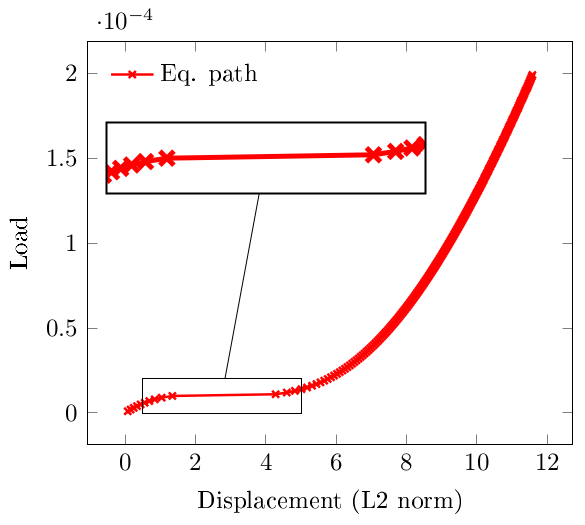
\includegraphics[width=0.7\textwidth]{crisfield_beam_eq_path.png}
%\caption{Equilibrium path}
%\end{figure}
%\end{column}
%\begin{column}{0.49\textwidth}
%\begin{figure}[h]
%\centering
%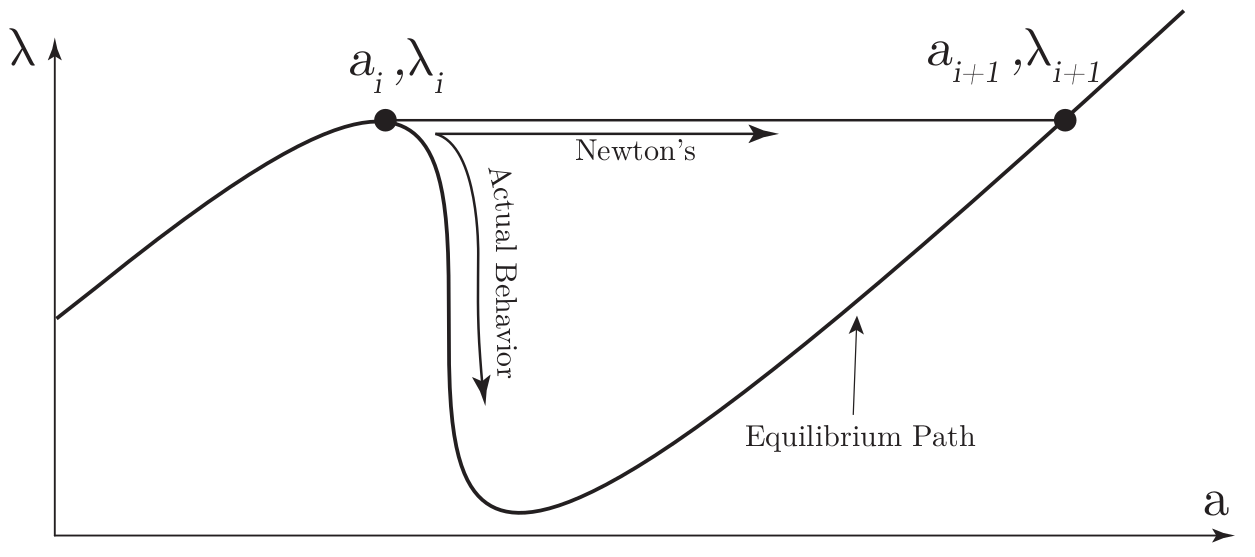
\includegraphics[width=0.85\textwidth]{newton_method_failure.png}
%\caption{Failure of Newton's method \cite{Vasios}}
%\end{figure}
%\end{column}
%\end{columns}
%}%
%\end{frame}

\subsection{Coupled problem}
\begin{frame}{Coupled problem set up}
\begin{columns}
\begin{column}{0.45\textwidth}
\begin{itemize}
\item Coupled PDE system: \\
$\text{Div}(\mathbb{B}) = 0$, \\
$\text{Div}(\mathbf{F} \cdot \mathbf{S}) + \mathbf{b}^p = \mathbf{0}$
\item Boundary conditions:\\ 
$\phi = \overline{\phi}$ on $\partial \mathcal{S}_{0,\phi}$,\\
$\mathbf{N} \cdot \llbracket \mathbb{B} \rrbracket = \overline{b}$ on $\partial \mathcal{S}_{0,B}$,\\
$\mathbf{u} = \mathbf{0}$ on $\partial \mathcal{S}_{0,\mathbf{u}}$, $ \llbracket \mathbf{F} \cdot \mathbf{S} \rrbracket \cdot \mathbf{N} = \mathbf{t}^p$ on $\partial\mathcal{B}_{0,t}$
\end{itemize}
\begin{figure}[h]
\centering
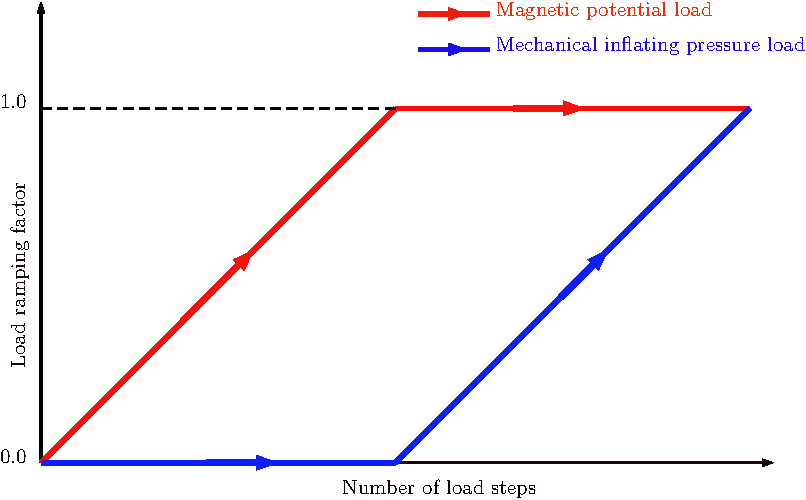
\includegraphics[width=0.98\textwidth]{load_cycle.pdf}
\caption{Load application cycle}
\end{figure}
\end{column}
\begin{column}{0.54\textwidth}
\begin{figure}[h]
\centering
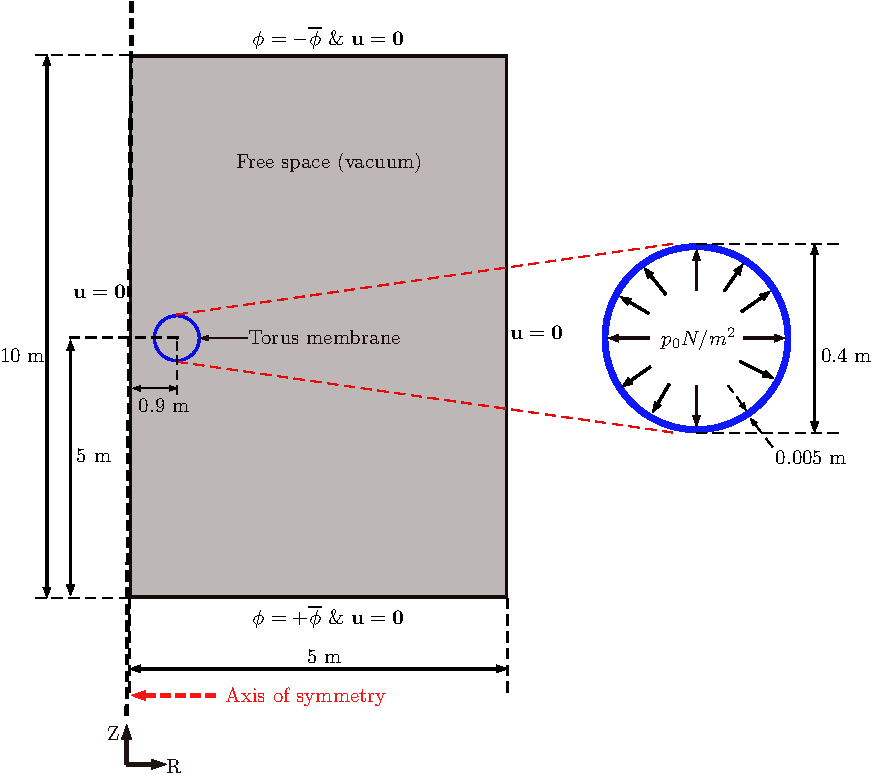
\includegraphics[width=0.9\textwidth]{coupled_prob_description.pdf}
\caption{Representative geometry description}
\end{figure}
\end{column}
\end{columns}
\end{frame}

\begin{frame}{Constitutive model for coupled problem}
\begin{itemize}
\item Hyperelastic material model for coupled magneto-elasticity:
\begin{empheq}[box=\tcbhighmath]{equation*}
\Psi(\mathbf{C},\mathbb{H}) \equiv \underbrace{\dfrac{\mu}{2} [\mathbf{C} : \mathbf{I} - \mathbf{I} : \mathbf{I} - 2 \ln J] + \dfrac{\lambda}{2} (\ln J)^2}_{\Psi^{\text{elas}}(\mathbf{C})} \underbrace{\alert{- \frac{\mu_0 \mu_r}{2} [J \mathbf{C}^{-1} : \mathbb{H} \otimes \mathbb{H}]}}_{\Psi^{\text{ME}}(\mathbf{C},\mathbb{H})},
\end{empheq}
\item First constitutive relation: $\mathbb{B} := -\dfrac{\partial \Psi (\mathbf{C},\mathbb{H})}{\partial \mathbb{H}}$
\item Second constitutive relation: $\mathbf{S} := 2 \dfrac{\partial \Psi (\mathbf{C},\mathbb{H})}{\partial \mathbf{C}}$
\end{itemize}
\end{frame}

\begin{frame}{Discretization by finite element method}
\begin{itemize}
\onslide<1-2>{
\item System of equations at load step $t_n$ and Newton iterate $i$:
\begin{equation*}
\begin{bmatrix}
\mathbf{K}_{\phi \phi} & \mathbf{K}_{\phi \mathbf{u}} \\
\mathbf{K}_{\mathbf{u} \phi} & \mathbf{K}_{\mathbf{u} \mathbf{u}}
\end{bmatrix}
\begin{bmatrix}
\Delta \mathbf{d}_{\phi} \\
\Delta \mathbf{d}_{\mathbf{u}}
\end{bmatrix}
=
\begin{bmatrix}
-\mathbf{R}_{\phi} \\
-\mathbf{R}_{\mathbf{u}}
\end{bmatrix}
\implies \ \mathbf{K} \cdot \Delta \mathbf{d} = \mathbf{f} \ \ \text{\alert{Saddle point system}}
\end{equation*}
\item Solution update: $\mathbf{d}_{i+1}^n = \mathbf{d}_i^n + \Delta \mathbf{d}^n$\\
}%
\onslide<2>{
\begin{columns}
\begin{column}{0.6\textwidth}
\tiny{
\begin{align*}
K_{\phi \phi} = &- \sum\limits_q \left[ \nabla_0 N_I (q) \cdot \mathbf{D} \cdot \nabla_0 N_J (q) \right] \ \alpha \ J \ w(q) \nonumber \\
K_{\mathbf{u} \mathbf{u}} = & \sum\limits_q \left[ \left[ \nabla_0 \mathbf{N}_I^T (q) \cdot \nabla_0 \mathbf{N}_J (q) \right]^{\text{sym}} : \mathbf{S} \right]  \ \alpha \ J \ w(q) \nonumber \\
&+ \sum\limits_q \left[ \left[ \mathbf{F}^T \cdot \nabla_0 \mathbf{N}_I (q) \right]^{\text{sym}} : \mathfrak{C} : \left[ \mathbf{F}^T \cdot \nabla_0 \mathbf{N}_J (q) \right]^{\text{sym}} \right] \ \alpha \ J \ w(q), \nonumber\\
K_{\phi \mathbf{u}} = & \sum\limits_q \left[ \left[ \mathbf{F}^T \cdot \nabla_0 \mathbf{N}_I (q) \right] : \mathbb{P} \cdot \nabla_0 N_J (q) \right] \ \alpha \ J \ w(q) \nonumber \vspace{0.1cm}\\
& \text{with } \alpha = 2 \pi R.
\end{align*}
}
\end{column}
\begin{column}{0.39\textwidth}
\begin{itemize}
\item Elastic material tangent $\mathfrak{C} := 4\dfrac{\partial^2 \Psi (\mathbf{C}, \mathbb{H})}{\partial \mathbf{C} \otimes \partial \mathbf{C}}$
\item Magneto-static tangent $\mathbf{D} := -\dfrac{\partial^2 \Psi (\mathbf{C}, \mathbb{H})}{\partial \mathbb{H} \otimes \partial \mathbb{H}}$
\item Magneto-elasticity tangent $\mathbb{P} := -2 \dfrac{\partial^2 \Psi (\mathbf{C}, \mathbb{H})}{\partial \mathbf{C} \otimes \mathbb{H}}$ \\
$\mathbb{P}^T := -2 \dfrac{\partial^2 \Psi (\mathbf{C}, \mathbb{H})}{\partial \mathbb{H} \otimes \partial \mathbf{C}}$
\end{itemize}
\end{column}
\end{columns}
}%
\end{itemize}
\end{frame}

\begin{frame}{Results for coupled problem}
\only<1>{
Applied potential difference per unit length = $3.5e^5$
\begin{figure}[h]
\centering
\begin{subfigure}{0.32\textwidth}
\centering
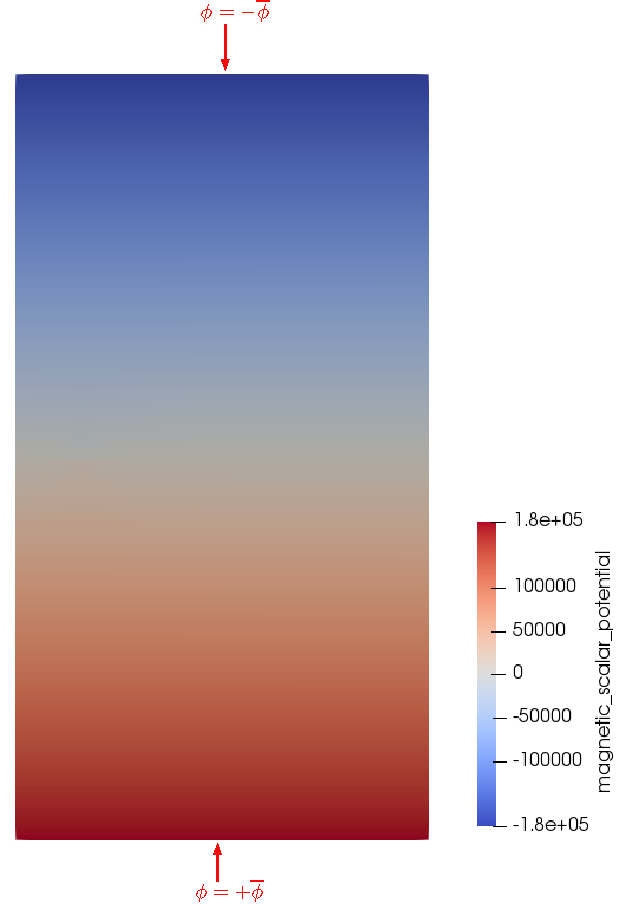
\includegraphics[width=0.9\textwidth]{magnetic_potential_coupled_problem.pdf}
\caption{Applied potential difference}
\end{subfigure}
\begin{subfigure}{0.32\textwidth}
\centering
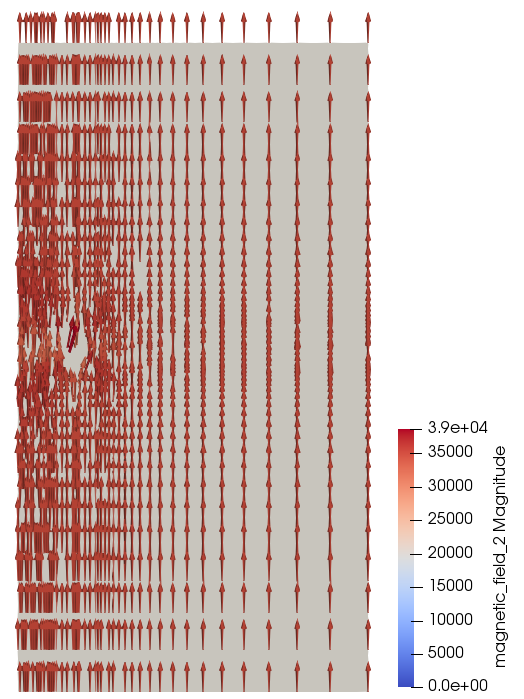
\includegraphics[width=0.9\textwidth]{magnetic_field_50.png}
\caption{Uniformly distributed magnetic field}
\end{subfigure}
\begin{subfigure}{0.32\textwidth}
\centering
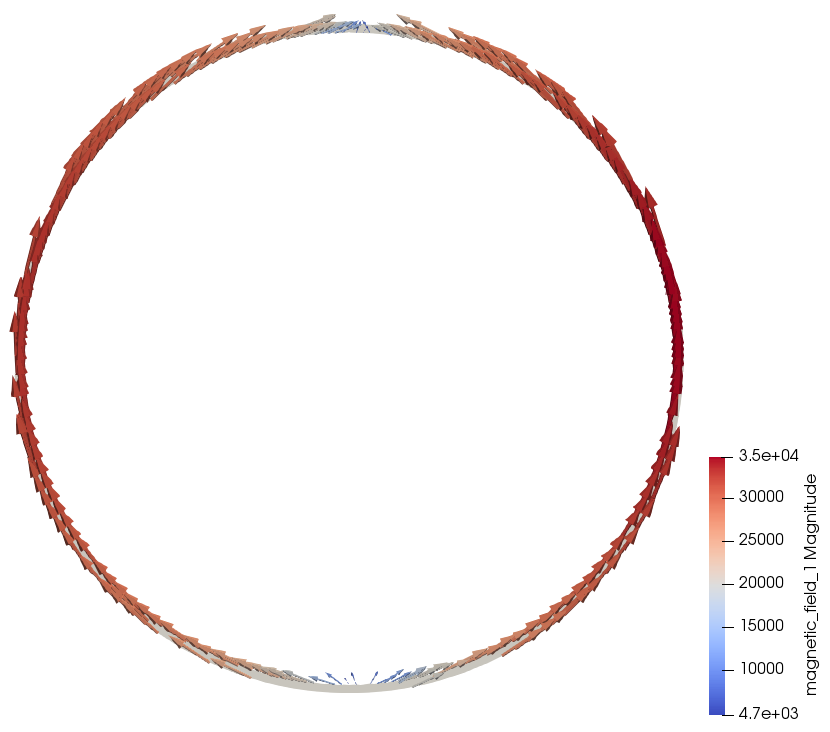
\includegraphics[width=0.9\textwidth]{magnetic_field_toroid_coupled.png}
\caption{Distribution of $\mathbb{H}$ in torus membrane}
\end{subfigure}
\end{figure}
}%
\only<2>{
Potential difference = $3.5e^5$, Inflating pressure load = 1500 Pa
\begin{figure}[h]
\centering 
\movie[width=8cm,height=7cm,poster,showcontrols]{}{new_coupled_deform_torus.avi}
\caption*{Finite deformations for coupled problem \alert{(Click image!)}}
\end{figure}
}%
\end{frame}

\section{Modelling of instabilities for coupled problem}
\begin{frame}{Modelling of instabilities in membrane}
\only<1>{
\begin{figure}[h]
\centering
\begin{subfigure}{0.3\textwidth}
\centering
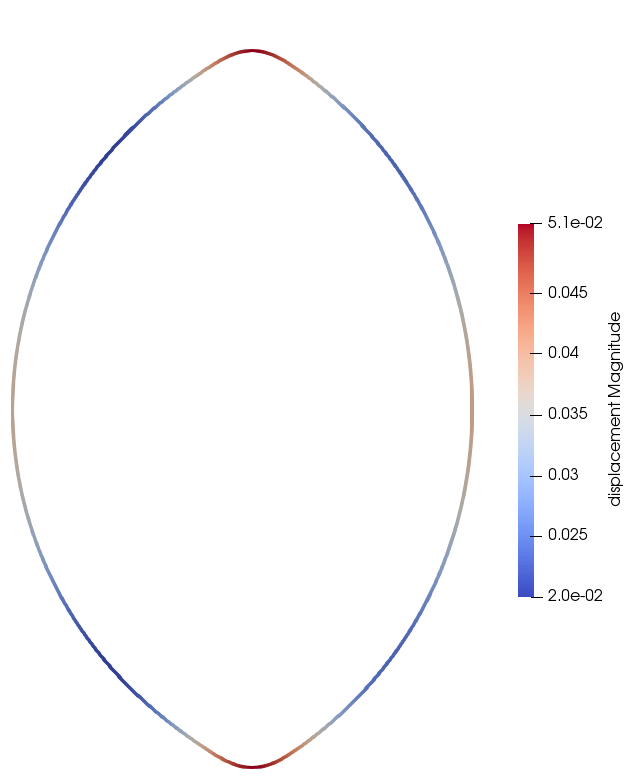
\includegraphics[width=0.85\textwidth]{instab_test_1_before_failure.png}
\caption{Before numerical failure}
\end{subfigure}
\begin{subfigure}{0.3\textwidth}
\centering
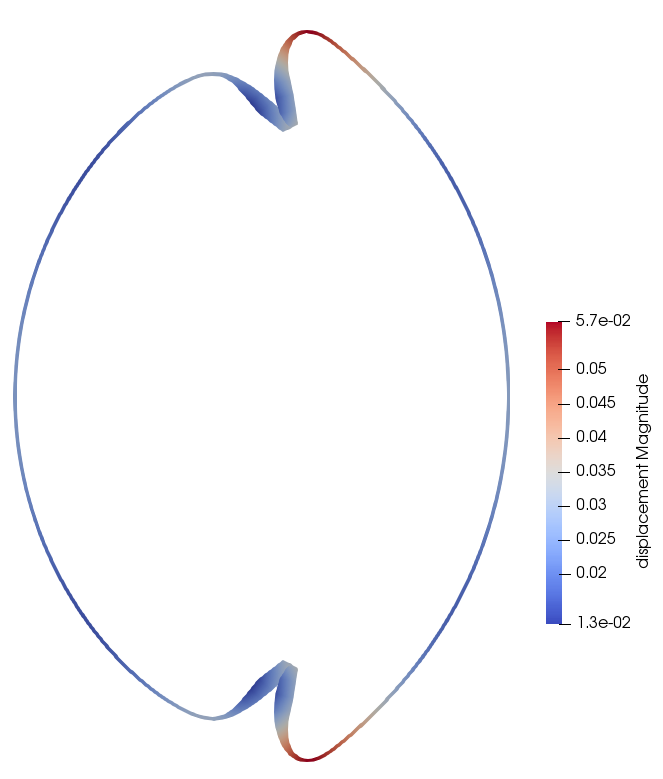
\includegraphics[width=0.9\textwidth]{instab_test_1_membrane_inv_cells.png}
\caption{After numerical failure}
\end{subfigure}
\begin{subfigure}{0.38\textwidth}
\centering
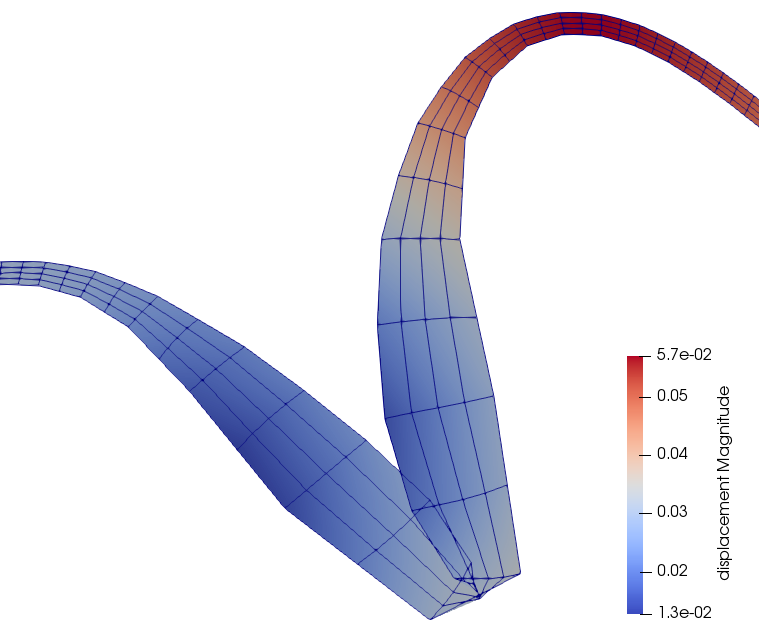
\includegraphics[width=0.9\textwidth]{instab_test_1_membrane_disp.png}
\caption{Zoomed view of inverted elements in membrane}
\end{subfigure}
\caption{Magneto-elastic membrane during numerical failure}
\end{figure}
\begin{center}
\alert{Numerical artefact before observing any unstable deformation of the membrane!}
\end{center}
}%
\only<2>{
\begin{figure}[h]
\centering
\begin{subfigure}{0.4\textwidth}
\centering
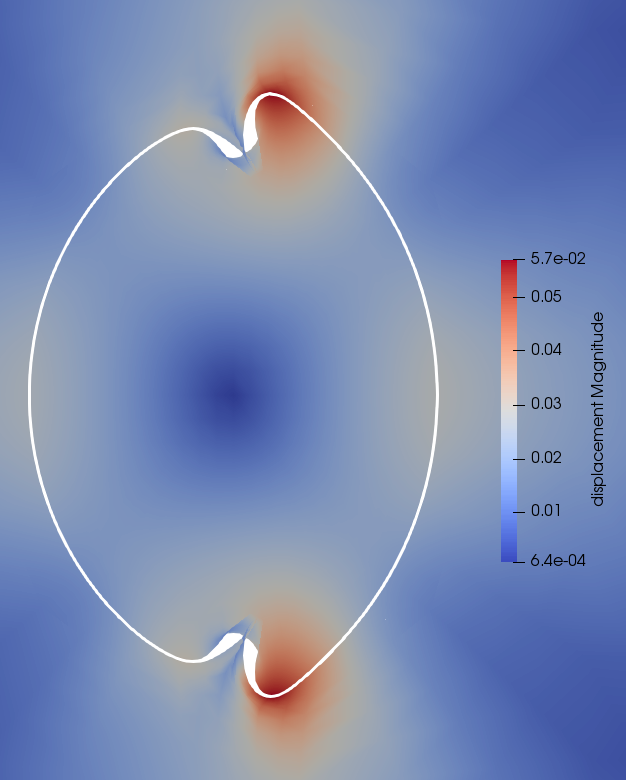
\includegraphics[width=0.9\textwidth]{instab_test_1_inv_cells.png}
\caption{After numerical failure}
\end{subfigure}
\begin{subfigure}{0.58\textwidth}
\centering
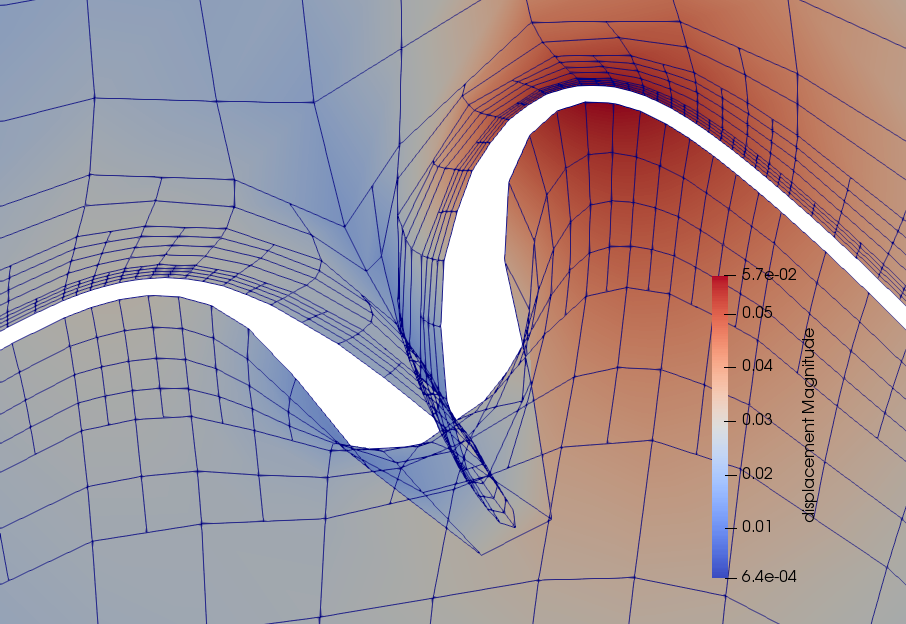
\includegraphics[width=0.9\textwidth]{instab_test_1_free_space_inv_cells.png}
\caption{Zoomed view of inverted elements in free space}
\end{subfigure}
\caption{Free space elements surrounding the membrane causing the numerical failure (white section is the cut-out membrane for better visualization purpose)}
\end{figure}
\vspace{-3em}
\begin{columns}
\begin{column}{0.4\textwidth}
\begin{align*}
\Psi &= \Psi^{\text{elas}}(\mathbf{C}) + \Psi^{\text{ME}}(\mathbf{C},\mathbb{H}) \\
\mathfrak{C} &= \mathfrak{C}^{\text{elas}}(\mathbf{C}) + \mathfrak{C}^{\text{ME}}(\mathbf{C},\mathbb{H})
\end{align*}
\end{column}
\begin{column}{0.59\textwidth}
\begin{center}
\alert{Need to implement mesh-update technique!}
\end{center}
\end{column}
\end{columns}
}%
\end{frame}

% Placing a * after \section means it will not show in the
% outline or table of contents.
\section*{Summary}

\begin{frame}{Summary}
  \begin{itemize}
  \item A robust framework for multi-physics magneto-elasticity problems was developed
  \item Axisymmetric solids with axisymmetric loads and boundary conditions were particularly focussed
  \item An attempt to model the unstable deformations in membrane near the limit points was made
  \end{itemize}
  
  \begin{itemize}
  \item
    Outlook
    \begin{itemize}
    \item Implement a `mesh-update technique' and solve the coupled problem with segregated modelling approach
    \item Get the Arc-Length method to function correctly
    \item Employ other constitutive material models such as Mooney-Rivlin along with the incompressiblity condition
    \end{itemize}
  \end{itemize}
\end{frame}

\begin{frame}{References}
\printbibliography
\end{frame}

\begin{frame}
\centering
\Large Thank you for your attention! \\
\vspace{1cm}
Any questions?
\end{frame}

\end{document}


